% !Mode:: "TeX:UTF-8"

\documentclass[authordraft]{ctacn}

\usepackage{graphicx}
\usepackage{array}
\usepackage{multirow}
\usepackage{threeparttable}
\usepackage{capt-of}
\usepackage{float}
\usepackage{hhline}

\graphicspath{
  {../results/baseline/01b_equal_lookahead/}
  {../results/baseline/01b_equal_lookahead/subfigs/}
  {../results/baseline/02c_path_generalization_v4/}
  {../results/baseline/03_monte_carlo/}
  {../results/baseline/04_parameter_sensitivity/}
  {../results/baseline/05b_ablation_v2/subfigs/}
  {tikz/}
}

\newcommand{\journaltable}{\zihao{6}\setlength{\tabcolsep}{3.5pt}\renewcommand{\arraystretch}{1.15}}
\newcolumntype{C}{>{\centering\arraybackslash}c}
\setlength{\abovecaptionskip}{3pt}
\setlength{\belowcaptionskip}{4pt}
\makeatletter
\setlength{\@fptop}{0pt}
\setlength{\@fpsep}{8pt plus 2pt}
\setlength{\@fpbot}{0pt plus 1fil}
\makeatother

\allowdisplaybreaks[4]

\begin{document}

\Volume{xxxx}{x}{xxx}{xx}{x}
\cndoi{1001-0920(0000)00-0000-00}
\doi{\zihao{-5}10.13195/j.kzyjc.2026.0000}
\paperdate{2026-xx-xx}{2026-xx-xx}
\setcounter{page}{1}
\osid{}

\runheading{面向无人艇航点路径跟踪的速度-航向协同整形控制}
\xiangmujijin{}
\zerenbianwei{编委1.}
\authorcor{E-mail: zuozheyi@163.com.}

\cntitle{面向无人艇航点折线路径跟踪的速度-航向协同整形控制}

\cnauthor{作者一\makebox{$^{1,2\dag}$},~~作~~~~者\makebox{$^{1}$}}
{(1. 作者单位1~二级单位，省份~城市~邮编；2. 作者单位2~二级单位，省份~城市~邮编)}

\cnabstract{针对欠驱动无人水面艇沿航点折线路径航行时，LOS-PID 分层结构在航段切换处容易产生航向参考突变，并诱发偏航力矩饱和、积分卷绕及双桨推进余量竞争等问题，提出一种速度-航向协同整形（speed-heading co-shaping, SHCS）控制方法。该方法不改变原有 ILOS-PID 主体框架，而是在导引律与底层 PID 控制器之间引入参考通道整形层：一方面，依据 CyberShip II 偏航动力学与双桨偏航力矩约束构造动态航向整形器，将几何期望航向转化为满足执行器可达性的参考航向；另一方面，基于航向整形残差和推进器联合约束调度期望纵荡速度，以在转弯阶段协调偏航控制与纵荡推进资源。基于统一配置与可复现实验脚本的仿真结果表明，在统一前视距离（$\Delta=4$ m）条件下，与 ILOS-PID 相比，SHCS 典型 L 形路径定常海流场景下 CTE-RMS 仅增大约 6.7\%，同时将偏航控制能耗降低 23.2\% 并消除执行器饱和（0.65~s 降为 0）；固定速率整形（FR）和一阶参考模型（FO）虽同样消除饱和，但 CTE-RMS 分别恶化 302\% 和 238\%，说明 SHCS 能在接近 ILOS-PID 跟踪精度的前提下实现饱和抑制和能耗节省。在以 Z 形和 U 形为代表性路径、覆盖三种工况的 6 个泛化场景中，所提方法均进入 3 m 目标容差圆，偏航能耗改善 21.3\%--31.8\%，CTE-RMS 在无扰动工况下基本持平（$-0.6\%$\,--\,$+1.4\%$），定常海流工况下略有增大（$2.7\%$\,--\,$10.3\%$），含噪海流工况下进一步增大（$13.6\%$\,--\,$19.1\%$）；在 30 个随机化配对蒙特卡洛工况下，SHCS 以约 19.6\% 的横向误差 RMS 代价换取偏航控制能耗和原始偏航饱和时间分别降低 27.8\% 和 95.1\%。}

\cnkeyword{无人艇；路径跟踪；积分视线导引；航向参考整形；速度调度；蒙特卡洛验证}
\clc{}
\wenxianbiaoshi{A}

\entitle{Speed-heading co-shaping control for waypoint path following of unmanned surface vehicles}

\enauthor{ZUO Zhe-yi\makebox{$^{1,2\dag}$},~~ZUO Zhe\makebox{$^{1}$}}
{(1. College of Information Science and Engineering, Northeastern University, Shenyang~110004, China; 2. College of Engineering, Qufu Normal University, Rizhao~276826, China)}

\enabstract{Waypoint-path following of underactuated unmanned surface vehicles is often implemented by a line-of-sight guidance law cascaded with PID controllers. At waypoint transitions, however, the geometric heading command may change abruptly and consequently cause yaw-moment saturation, integral windup, and competition for the limited twin-thruster margin. To address this reference feasibility problem, this paper proposes a speed-heading co-shaping (SHCS) control method. Without modifying the basic ILOS-PID architecture, SHCS inserts a reference-channel layer between guidance and control. The proposed layer consists of a dynamic heading shaper, which converts the geometric ILOS command into an executable heading reference according to the CyberShip II yaw dynamics and yaw-moment constraint, and a velocity scheduler, which adjusts the desired surge speed using the shaping residual and the joint thruster constraint. Under a common lookahead distance ($\Delta=4$~m), reproducible simulations show that SHCS increases the cross-track-error RMS by only 6.7\% relative to ILOS-PID in a typical L-shape path under steady current, while reducing yaw-control energy by 23.2\% and eliminating saturation entirely (from 0.65~s to zero). Fixed-rate shaping (FR) and first-order reference model (FO) also eliminate saturation but degrade cross-track-error RMS by 302\% and 238\%, respectively, demonstrating that SHCS achieves saturation suppression and energy saving with near-baseline tracking accuracy. In six generalization scenarios covering Z-shape and U-shape representative paths under three disturbance conditions, SHCS reaches the 3~m goal tolerance in all cases, improves yaw-control energy by 21.3\%--31.8\%, keeps cross-track-error RMS within $-0.6\%$ to $+1.4\%$ of the ILOS-PID baseline in calm conditions, within $2.7\%$--$10.3\%$ in steady-current conditions, and within $13.6\%$--$19.1\%$ in noisy-current conditions. In 30 randomized paired Monte Carlo cases, SHCS trades a 19.6\% increase in cross-track-error RMS for reductions of 27.8\% and 95.1\% in yaw-control energy and raw saturation time, respectively.}

\enkeyword{unmanned surface vehicle; path following; integral line-of-sight guidance; heading reference shaping; velocity scheduling; Monte Carlo validation}

\maketitle

\begin{multicols}{2}

\section{引\quad 言}

无人水面艇（unmanned surface vehicle, USV）能够在海洋测绘、港口巡检、应急搜救和近岸安防等任务中执行长时间自主航行，其轨迹通常由离散航点序列或分段路径给定。路径跟踪控制的核心目标是在海流扰动、模型不确定性和执行器约束共同作用下，使艇体以可接受的横向误差、控制能耗和执行器负荷跟踪参考路径。视线导引（line-of-sight, LOS）及其积分扩展形式 ILOS 因结构清晰、参数物理意义明确且便于工程实现，常与速度/航向 PID 控制器构成分层路径跟踪系统\textsuperscript{[3,5-7]}。

对于由航点连接形成的折线路径，航段切换会使路径方位角发生离散变化，从而导致 LOS 几何期望航向 $\psi_d$ 出现近似阶跃的参考变化。若该命令直接输入航向 PID 控制器，双桨欠驱动 USV 中将出现两类相互耦合的约束效应：其一，原始偏航力矩命令可能超过最大可实现偏航力矩，造成执行器饱和并诱发积分卷绕；其二，偏航通道会占用双桨推进器可行域，使可用于纵荡推进的余量下降，进而影响转弯阶段的速度维持、能量分配和横向误差收敛。
因此，折线路径跟踪中的关键问题不仅是导引参数或 PID 增益整定，还包括导引参考在底层执行器约束下的可执行性。若缺少参考通道层面的约束处理，短前视距离虽然可能提升几何跟踪积极性，却也会放大航段切换处的航向突变和偏航控制压力。

现有研究主要从三类途径缓解上述矛盾。第一类是导引律改进，例如 ILOS、自适应 LOS 或曲线路径参数化方法，它们能够降低定常海流引起的稳态横向误差，但通常不直接约束航段切换时的航向参考变化率\textsuperscript{[6-8]}。第二类是在参考通道加入一阶滤波或固定速率限幅，该类方法实现简单，但时间常数或限幅阈值多为预设常数，难以根据当前偏航速率、推进器余量和转弯强度自适应调整。第三类是采用控制分配或模型预测控制显式处理执行器约束，其理论框架更完整，但对模型精度、在线优化和工程部署条件提出了更高要求\textsuperscript{[10,12]}。对于已经采用 ILOS-PID 的工程系统，可在导引律与底层控制器之间构造独立的可执行参考生成机制，以保留原有分层控制框架。

基于上述考虑，本文提出速度-航向协同整形（speed-heading co-shaping, SHCS）方法。SHCS 不替换 ILOS 导引律和 PID 控制器，而是在二者之间加入参考通道中间层：动态航向整形器依据偏航动力学可达性将几何期望航向 $\psi_d$ 转化为可执行参考航向 $\psi_{ref}$；速度调度器根据航向整形残差和推进器联合约束动态调整期望纵荡速度 $u_d$，从而在转弯过程中缓解偏航控制与纵荡推进之间的资源竞争。该设计试图在短前视 LOS 的几何跟踪能力与执行器约束下的参考平滑性之间建立折中。

本文的主要贡献如下：
1）面向双桨欠驱动 USV，揭示折线路径航段切换导致 LOS-PID 偏航饱和与推进余量竞争的机理，并将其形式化为参考通道可执行化问题；
2）提出一种基于偏航动力学可达性的动态航向整形器，使航向参考变化率随当前偏航状态和执行器能力自适应调整；
3）设计融合航向整形残差与推进器联合约束的速度调度层，并在保留原有 PID 控制器主体结构的基础上实现参考通道协同；
4）构建统一配置下的典型场景、多路径泛化、随机化配对蒙特卡洛、参数敏感性和消融实验协议，验证所提方法在横向误差、控制能耗和执行器饱和之间形成的可复现折中关系。

\section{问题建模}
\subsection{USV 模型与双桨约束}
采用惯性坐标系描述位置与艏向角，状态向量记为 $\boldsymbol{\eta}=[x,y,\psi]^{\mathrm T}$，
船体坐标系速度记为 $\boldsymbol{\nu}=[u,v,r]^{\mathrm T}$。
三自由度运动学方程为
\begin{equation}
\dot{\boldsymbol{\eta}}=\boldsymbol{J}(\psi)\boldsymbol{\nu},
\quad
\boldsymbol{J}(\psi)=
\begin{bmatrix}
\cos\psi & -\sin\psi & 0\\
\sin\psi &  \cos\psi & 0\\
0 & 0 & 1
\end{bmatrix}.
\label{eq:kinematics}
\end{equation}
忽略纵摇、横摇和升沉运动后，水平面三自由度动力学可写为
\begin{equation}
\boldsymbol{M}\dot{\boldsymbol{\nu}}
+\boldsymbol{C}(\boldsymbol{\nu})\boldsymbol{\nu}
+\boldsymbol{D}(\boldsymbol{\nu})\boldsymbol{\nu}
=\boldsymbol{\tau},
\label{eq:dynamics}
\end{equation}
其中 $\boldsymbol{M}$ 为刚体质量与附加质量矩阵，$\boldsymbol{C}(\boldsymbol{\nu})$ 为科氏及向心矩阵，$\boldsymbol{D}(\boldsymbol{\nu})$ 为阻尼矩阵。考虑欠驱动双桨 USV 不具备独立横荡执行器，控制输入取为 $\boldsymbol{\tau}=[\tau_u,0,\tau_r]^{\mathrm T}$，其中 $\tau_u$ 和 $\tau_r$ 分别表示纵荡推力与偏航力矩。

双桨推进器的左、右推力 $T_L,T_R$ 与广义力满足
\begin{equation}
\tau_u=T_L+T_R,\qquad
\tau_r=\frac{b}{2}(T_R-T_L).
\label{eq:thruster_map}
\end{equation}
当 $|T_L|,|T_R|\leq T_{\max}$ 时，由式（\ref{eq:thruster_map}）可得纵荡与偏航通道的菱形联合约束
\begin{equation}
|\tau_u|+\frac{2}{b}|\tau_r|\leq 2T_{\max}.
\label{eq:joint_constraint}
\end{equation}
式（\ref{eq:joint_constraint}）说明，偏航力矩需求越大，可用于纵荡推进的余量越小。因此，折线转弯阶段的执行器受限并非单一航向通道问题，而是偏航控制与纵荡推进在同一双桨可行域内共享资源的问题。对于后续采用的 CyberShip II 双桨参数，最大可达偏航力矩为 $\tau_{r,\max}=9$ N$\cdot$m，该约束关系构成速度-航向协同整形的物理基础。

\subsection{LOS导引与航段切换}
视线法（LOS）根据无人艇当前位置与路径前视点的几何关系生成期望航迹角\textsuperscript{[5]}。其基本几何关系如图~\ref{fig:los} 所示。
\begin{center}
	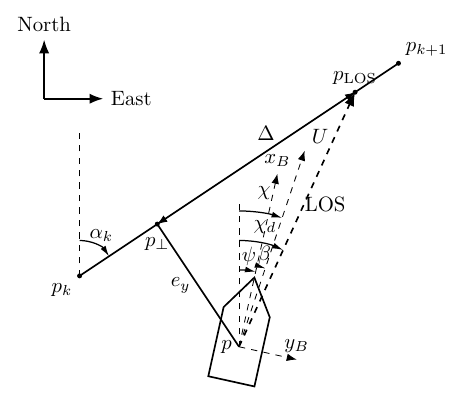
\includegraphics[width=0.9\columnwidth]{los_tiny.png}\\
	\figcaption{LOS导引几何关系示意图}
	\label{fig:los}
\end{center}
对于由航点序列构成的折线路径，设当前路径段方位角为 $\alpha_k$，无人艇相对于路径的横向误差为 $e_{ct}$，前视距离为 $\Delta$，则经典 LOS 导引律可表示为
\begin{equation}
\chi_d=\alpha_k+\arctan\!\left(-\frac{e_{ct}}{\Delta}\right),
\label{eq:los}
\end{equation}
其中 $\chi_d$ 为期望航迹角。严格而言，LOS 几何关系直接给出的是航迹角而非艏向角；若显式考虑侧滑角 $\beta$，则输入艏向控制器的参考应为 $\psi_d=\chi_d-\beta$。本文未单独引入侧滑角观测器，而是利用 ILOS 积分项补偿定常海流引起的稳态横向偏差，因此在控制实现中取 $\psi_d=\chi_d$。下文所称期望航向 $\psi_d$ 均指输入航向控制器的期望艏向参考。

在定常海流扰动下，经典 LOS 可能存在非零稳态横向误差。积分 LOS（ILOS）在经典 LOS 基础上引入横向误差积分项，以持续补偿由海流引起的稳态偏流\textsuperscript{[6,7]}。因此，本文选用 ILOS 作为基础导引律。

对当前路径段，令 $\psi_p=\alpha_k$，其期望航向可写为
\begin{equation}
\psi_d=\psi_p+\arctan\!\left(-\frac{e_{ct}+\sigma_i}{\Delta}\right),
\label{eq:ilos}
\end{equation}
其中
$\sigma_i$ 为 ILOS 积分状态。由式（\ref{eq:ilos}）可见，较小前视距离 $\Delta$ 能提高导引律对横向误差的响应速度，但也会放大航段切换或误差突变时的航向参考变化。

以 90$^\circ$ 折线转弯为例，航段切换时几何期望航向变化量近似为 $\Delta\psi_d=\pi/2$。若该变化直接进入航向 PID 比例环节，按本文仿真采用的比例增益 $K_p=30$ 估计，瞬时名义偏航力矩约为 $K_p\Delta\psi_d\approx47$ N$\cdot$m，明显超过 CyberShip II 的可用偏航力矩上限。因此，即使 ILOS 能够补偿定常海流引起的稳态横向偏差，折线路径航段切换处仍可能出现参考命令与执行能力不匹配的问题。

据此，本文的控制目标是在双桨推进器约束下保持路径跟踪精度，降低航段切换时的航向参考不可执行程度，抑制偏航饱和及积分卷绕，并在转弯阶段协调纵荡推进与偏航控制资源。因此，后续 SHCS 设计将把 ILOS 输出视为几何期望命令，并在其进入 PID 控制器前进行可执行化处理。
\section{速度-航向协同整形方法}

\subsection{总体结构}
为抑制折线路径航段切换引起的偏航饱和、积分卷绕和推进余量竞争，本文在 ILOS 导引律与 PID 控制器之间引入速度-航向协同整形（SHCS）层。该层由动态航向参考整形器和速度调度器构成，其作用不是重新设计底层控制律，而是在参考通道中生成更符合执行器约束的航向和速度命令。

所提方法的总体结构如图~\ref{fig:architecture} 所示。

原始 ILOS-PID 结构可表示为“路径点 $\rightarrow$ ILOS $\rightarrow$ 航向/速度 PID $\rightarrow$ 双桨推进器 $\rightarrow$ USV”。SHCS 在 ILOS 与 PID 之间加入两类参考修正：动态航向整形层输出可执行航向参考 $\psi_{ref}$，速度调度层输出期望纵荡速度 $u_d(t)$。底层仍采用原有速度 PID 和航向 PID，双桨分配器仍按照式（\ref{eq:joint_constraint}）施加物理约束。因此，SHCS 可在保留既有 LOS-PID 主体结构的基础上实现参考通道约束处理。

\end{multicols}
\begin{center}
	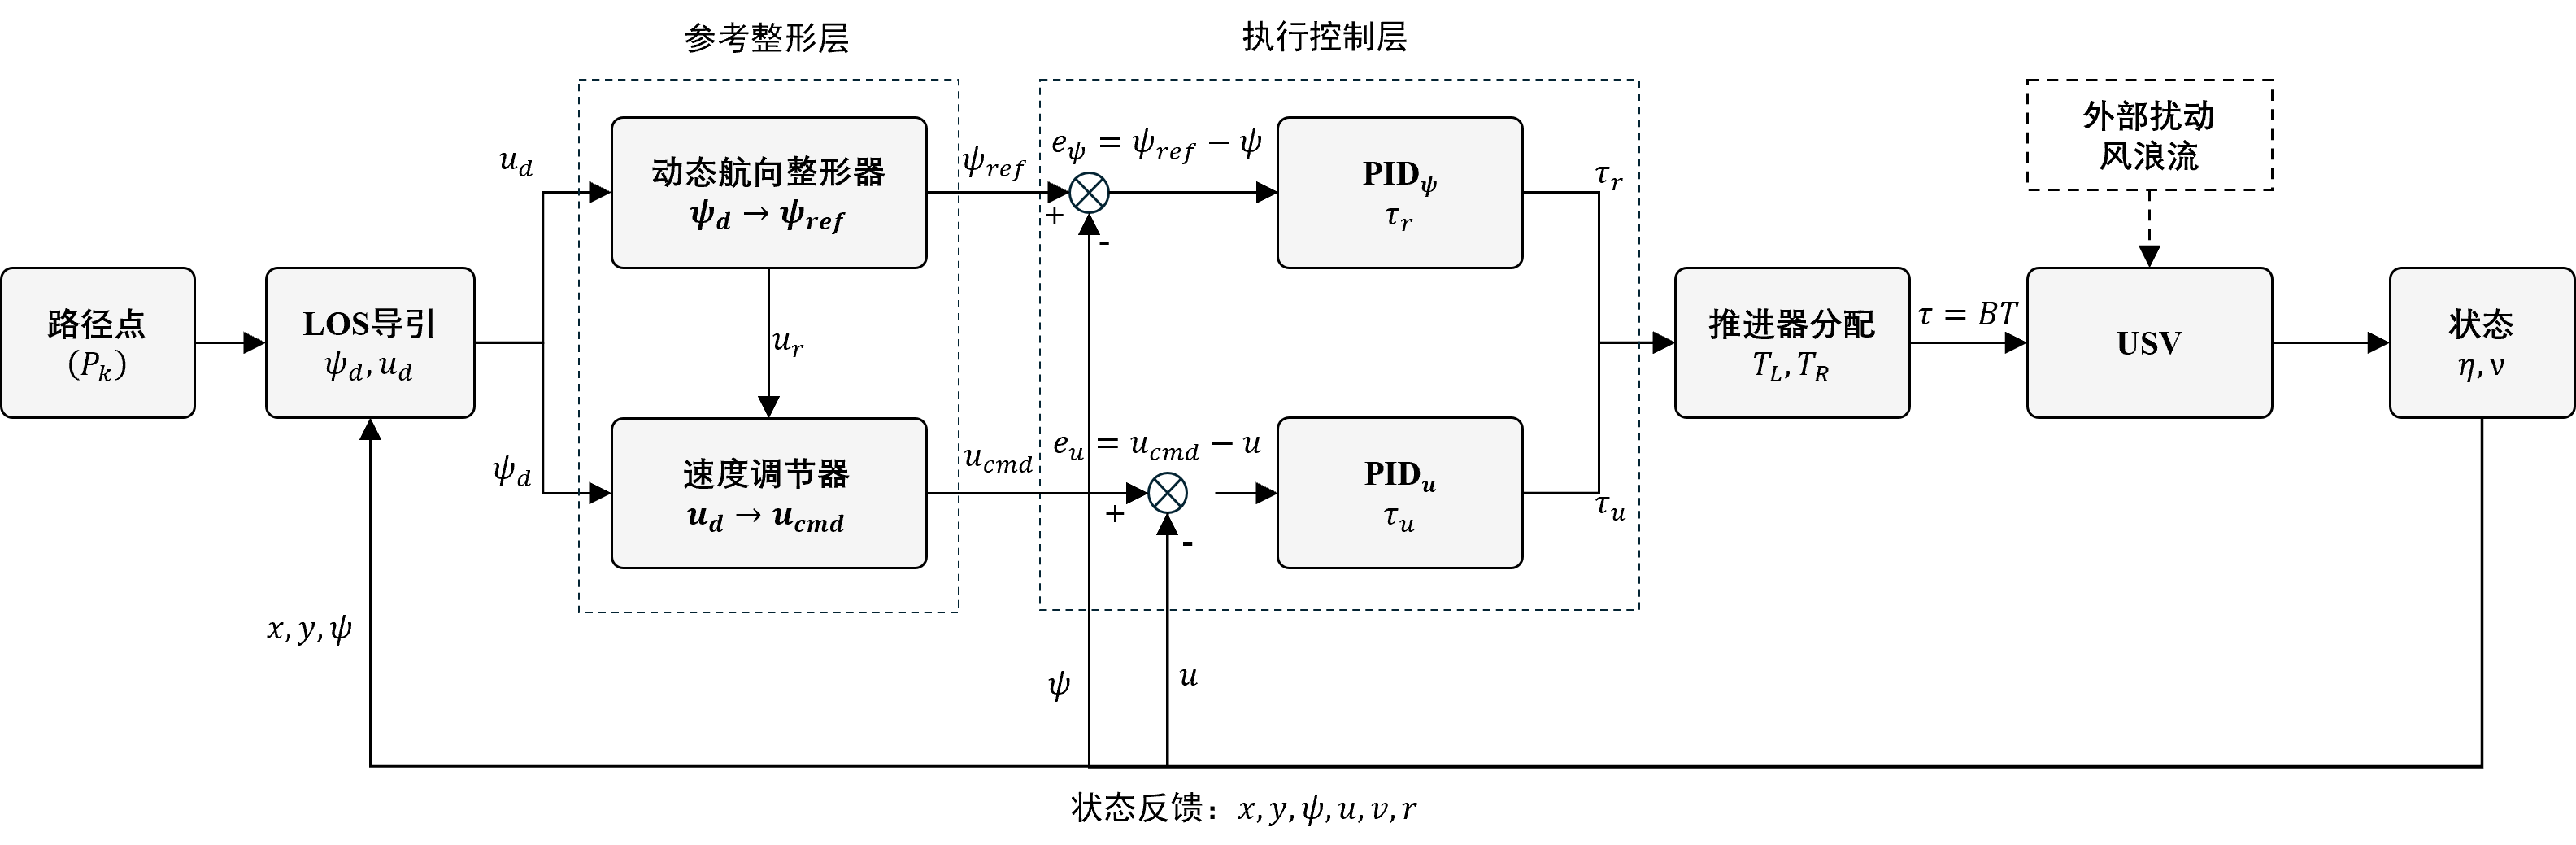
\includegraphics[width=0.9\textwidth]{control_architecture.png}\\
	\figcaption{SHCS 控制结构示意图}
	\label{fig:architecture}
\end{center}
\begin{multicols}{2}

\subsection{动态航向整形器}

动态航向整形器的输入为 ILOS 几何航向 $\psi_d$ 和当前偏航角速度 $r$，输出为参考航向 $\psi_{ref}$。其核心思想是根据当前偏航动力学状态估计短时可达的参考变化速率，而不是采用固定时间常数或固定速率阈值。由偏航单通道近似
\begin{equation}
M_{33}\dot r=\tau_r-N_r r-N_{rr}|r|r
\label{eq:yaw_channel}
\end{equation}
可得在最大偏航力矩作用下的一步最大角加速度估计
\begin{equation}
\dot r_{\max}(t)=
\frac{\max\{0,\tau_{r,\max}+N_r r+N_{rr}|r|r\}}{M_{33}}.
\label{eq:rdotmax}
\end{equation}
进一步考虑当前偏航速率和工程安全上限，定义整形速率上限为
\begin{equation}
r_{\lim}(t)=
\min\left\{r_{\mathrm{nom}},~|r(t)|+\dot r_{\max}(t)\Delta t\right\}.
\label{eq:rlim}
\end{equation}
随后对参考航向进行离散更新：
\begin{equation}
\begin{aligned}
\psi_{ref,k+1}=&~\psi_{ref,k}
+\mathrm{sat}_{[-r_{\lim},r_{\lim}]}\\
&\left(\frac{\mathrm{wrap}(\psi_{d,k}-\psi_{ref,k})}{\Delta t}\right)\Delta t .
\end{aligned}
\label{eq:shaper_update}
\end{equation}
其中 $\mathrm{wrap}(\cdot)$ 将角度误差映射至 $(-\pi,\pi]$，$\mathrm{sat}_{[-r_{\lim},r_{\lim}]}(\cdot)$ 表示速率限幅。与固定速率限幅相比，式（\ref{eq:rlim}）可随当前偏航状态调整参考变化速度；与一阶滤波相比，其参数具有更明确的物理含义，并直接关联执行器偏航力矩上限。

\subsection{速度调度层}

航向整形层的残差定义为
\begin{equation}
e_s(t)=\mathrm{wrap}(\psi_d(t)-\psi_{ref}(t)).
\label{eq:shaping_error}
\end{equation}
$|e_s|$ 越大，说明当前几何航向命令与可执行参考之间的差异越大，系统通常处于较强转弯或整形尚未完成的阶段。此时若仍维持较高纵荡速度，横向偏离和推进器余量竞争均可能加剧。为此，首先构造基于整形残差的简单（simple）模式速度调度律：
\begin{equation}
u_{d,\lambda}(t)=u_{\mathrm{nom}}
\left(1-\lambda\frac{\max(0,|e_s|-e_{\mathrm{db}})}
{e_{s,\max}-e_{\mathrm{db}}}\right),
\label{eq:simple_scheduler}
\end{equation}
并将其裁剪至 $[u_{\min},u_{\mathrm{nom}}]$。其中 $\lambda$ 为降速强度，$e_{\mathrm{db}}$ 为小误差死区，$e_{s,\max}$ 为归一化残差上界。该项使速度命令随航向整形压力连续下降，避免在小残差条件下产生不必要降速。

为进一步体现推进器联合约束，耦合（coupled）模式通过 PID 的只读 preview 接口估计本步偏航力矩需求 $\tau_r^{pre}$，但不更新 PID 的积分和微分内部状态。由式（\ref{eq:joint_constraint}）可得当前可用纵荡推力上界
\begin{equation}
\tau_{u,\mathrm{avail}}
=\max\left\{0,2T_{\max}-\frac{2}{b}|\tau_r^{pre}|\right\},
\label{eq:tauu_avail}
\end{equation}
对应速度上限
\begin{equation}
u_{d,\kappa}=u_{\mathrm{nom}}
\min\left\{1,\frac{\tau_{u,\mathrm{avail}}}{2T_{\max}}\right\}.
\label{eq:ud_kappa}
\end{equation}
完整 SHCS 取
\begin{equation}
u_d(t)=\mathrm{clip}\{\min(u_{d,\lambda},u_{d,\kappa}),
u_{\min},u_{\mathrm{nom}}\},
\label{eq:ud_final}
\end{equation}
并对 $u_d$ 进行一阶平滑和斜率限制，以避免速度命令突变。需要指出的是，整形残差项反映导引参考与可执行参考之间的动态不一致，推进器约束项反映偏航力矩对纵荡推力余量的占用，两者分别从参考层和执行器层刻画转弯压力。典型单转弯工况下耦合（coupled）调度与简单（simple）调度数值接近，说明整形残差信号已足以触发主要降速动作；coupled 项则为更强扰动或连续急转场景提供推进器约束感知能力。

\subsection{实现结构与复现实验流程}

为保证数值结果的可追溯性，本文采用配置驱动的仿真实现。统一配置文件给出船模参数、PID 增益、路径、扰动、整形器、速度调度器和实验协议；控制器模块依次串联 ILOS、航向整形器、速度调度器和 PID 控制器；仿真器模块负责 RK4 闭环积分、扰动注入、双桨分配和日志记录；指标模块统一计算 RMS、IAE、控制能耗、转弯窗口指标和统计检验。第 4 节中的典型场景、泛化实验、蒙特卡洛实验、参数敏感性分析和消融实验均由独立脚本调用同一配置源生成，从而减少人工整理数据带来的不一致风险。

\section{仿真验证}
本文选取 CyberShip II 作为仿真对象。该对象为挪威 NTNU Marine Cybernetics Laboratory 开发的 1:70 海工补给船缩比模型，船长约 1.255 m，质量约 23.8 kg。考虑本文关注水平面路径跟踪问题，仿真采用其三自由度操纵模型，仅描述纵荡、横荡和偏航运动；控制输入中不设置独立横荡执行器，仅保留纵向推力与偏航力矩输入，因此可作为等效欠驱动双桨 USV 模型。实验评价围绕路径跟踪精度、航向参考可执行性、控制能耗和执行器饱和等指标展开。
\subsection{实验设置}

仿真步长为 $\Delta t=0.05$ s，积分方法为四阶 Runge-Kutta（RK4），最长仿真时间为 200 s，初始状态为 $\boldsymbol{\eta}_0=[0,-10,0]^{\mathrm T}$、$\boldsymbol{\nu}_0=[0,0,0]^{\mathrm T}$。终点到达容差设为 3 m，与 ILOS 航点切换半径保持一致。为降低启动瞬态对稳态评价的影响，除特别说明外，指标统计从 15 s 后开始。额定纵荡速度为 $u_{\mathrm{nom}}=1.5$ m/s，最低调度速度为 $u_{\min}=0.3$ m/s，默认降速强度为 $\lambda=0.6$，默认整形速率安全上限为 $r_{\mathrm{nom}}=1.5$ rad/s。

本文所有对比实验均采用统一前视距离 $\Delta=4$ m，包括 ILOS-PID 基线。该设置使方法间差异完全来自参考整形和速度调度机制，而非前视距离选择。本文设置 3 类工况：无扰动 calm、定常海流 steady\_current（海流速度为 $[0.35,0.18]$ m/s）和含噪海流 current（在定常海流基础上加入力、控制、位姿和速度噪声）。典型场景、参数敏感性分析和消融实验采用 L 形路径与定常海流组合；泛化实验以 Z 形双折 90° 和 U 形折返为代表性路径，在上述 3 类工况下各验证一次，共形成 6 个泛化场景；蒙特卡洛实验采用 L 形路径，围绕含噪海流构造 30 个随机化配对工况。

\subsection{典型 L 形路径}

典型场景用于在统一前视距离（$\Delta=4$ m）下检验 SHCS 相对 ILOS-PID 的精度--执行器负荷折中特性。对比方法包括原始 ILOS-PID、固定速率整形 ILOS+FR、一阶整形 ILOS+FO 和完整 SHCS，所有方法均使用 $\Delta=4$ m。表~\ref{tab:typical} 给出关键指标。

\begin{center}
\tabcaption{典型 L 形路径定常海流场景各方法关键指标（所有方法均取 $\Delta=4$ m）}
\label{tab:typical}
\journaltable
\begin{threeparttable}
\begin{tabular}{@{}lCCCC@{}}
\hline
指标 & ILOS-PID & ILOS+FR & ILOS+FO & \textbf{SHCS} \\
\hline
CTE-RMS/m         & \textbf{0.8574}  & 3.4459  & 2.8937  & 0.9144 \\
转弯CTE/m         & \textbf{1.001}   & 4.6428  & 3.2193  & 1.219  \\
LOS航向RMS/rad$^{a}$ & \textbf{0.1367} & 0.3645 & 0.2466 & 0.1692 \\
偏航能耗$^{b}$    & 103.11  & 197.60  & 182.59  & \textbf{79.22}  \\
饱和时间/s        & 0.65    & 0.00    & 0.00    & \textbf{0.00}   \\
\hline
\end{tabular}
\begin{tablenotes}
\footnotesize
\item[$a$] LOS 航向 RMS 为几何 LOS 误差 $\psi_d - \psi$，对所有方法公平可比，不受整形层影响。
\item[$b$] 偏航能耗单位为 N$^2{\cdot}$m$^2{\cdot}$s（$\int\!\tau_r^2\,\mathrm{d}t$）。
\end{tablenotes}
\end{threeparttable}
\end{center}

\end{multicols}

\begin{center}
\includegraphics[width=0.98\textwidth]{fig2_composite.png}\\
\figcaption{典型L形路径方法对比}
\label{fig:typical}
\end{center}

\begin{multicols}{2}

表~\ref{tab:typical} 揭示了统一前视距离条件下各方法的精度--执行器负荷折中特性。ILOS-PID 具有最低的 CTE-RMS（0.8574 m）和 LOS 航向误差（0.1367 rad），但存在 0.65~s 饱和时间。FR 和 FO 通过固定参数滤波消除了饱和，但 CTE-RMS 分别恶化至 3.4459 m 和 2.8937 m，即相较 ILOS-PID 分别劣化 302\% 和 238\%，说明固定时间常数和速率阈值在消除饱和的同时严重损失了路径跟踪精度。SHCS 通过基于偏航动力学可达性的自适应整形，消除饱和（0.65~s 降为 0）并将偏航能耗从 103.11 降至 79.22（改善 23.2\%），同时 CTE-RMS 仅从 0.8574 m 增至 0.9144 m（增大 6.7\%）。图~\ref{fig:typical} 表明，ILOS-PID 在转弯附近出现明显力矩限幅压力，而 SHCS 通过航向整形使参考变化率自适应匹配执行器能力，并通过速度调度在转弯阶段降低 $u_d$，使推进器余量保持在合理范围内。相比之下，FR/FO 虽消除饱和，但过度平滑的参考导致 LOS 航向误差长时间积累，CTE 峰值显著高于 SHCS。

\subsection{多路径泛化性分析}

泛化实验选取两条代表性路径（Z 形双折 90° 与 U 形折返），在无扰动和定常海流两种工况下，对比 ILOS-PID 与 SHCS 的跟踪精度和偏航能耗特性。Z 形路径包含两次连续同向折弯，U 形路径包含一次折返场景，两者覆盖了多段折线路径中典型的折弯密度与几何拓扑差异。FR/FO 基线特性已在典型 L 形路径实验中得到充分刻画，本节聚焦 SHCS 与最强基线 ILOS-PID 的泛化对比。需要强调的是，本节并不以 SHCS 在 CTE-RMS 上全面优于 ILOS-PID 为判断标准；SHCS 的目标是在保持可接受路径误差的同时降低偏航能耗和执行器负荷。图~\ref{fig:generalization_traj} 给出两种工况下的轨迹对比，图~\ref{fig:generalization_metrics} 给出 CTE-RMS 与偏航能耗柱状图，表~\ref{tab:generalization} 汇总两条路径在全部三种工况下的折中数据。

\begin{center}
\includegraphics[width=\linewidth]{fig_traj_composite.png}\\
\figcaption{多路径泛化实验轨迹对比}
\label{fig:generalization_traj}
\end{center}

\begin{center}
\includegraphics[width=\linewidth]{fig_metrics.png}\\
\figcaption{多路径泛化实验指标对比}
\label{fig:generalization_metrics}
\end{center}

\begin{center}
\tabcaption{多路径泛化场景下的精度--能耗折中}
\label{tab:generalization}
\journaltable
\setlength{\tabcolsep}{3.0pt}
\begin{tabular}{@{}llCC@{}}
\hline
工况 & 路径 & CTE代价 & 能耗降低 \\
\hline
\multirow{2}{*}{无扰动}
  & Z形（双折）& $-0.6\%$ & $21.3\%$ \\
  & U形折返    & $+1.4\%$ & $23.6\%$ \\
\hline
\multirow{2}{*}{定常海流}
  & Z形（双折）& $+10.3\%$ & $22.1\%$ \\
  & U形折返    & $+2.7\%$  & $24.8\%$ \\
\hline
\multirow{2}{*}{含噪海流}
  & Z形（双折）& $+19.1\%$ & $31.5\%$ \\
  & U形折返    & $+13.6\%$ & $31.8\%$ \\
\hline
\end{tabular}

\vspace{2pt}
\parbox{0.96\linewidth}{\footnotesize
注：CTE代价定义为 $(\mathrm{CTE}_{\mathrm{SHCS}}-\mathrm{CTE}_{\mathrm{ILOS}})/\mathrm{CTE}_{\mathrm{ILOS}}$，正值表示 CTE-RMS 增大，负值表示 SHCS 略优；能耗降低定义为 $(E_{\mathrm{ILOS}}-E_{\mathrm{SHCS}})/E_{\mathrm{ILOS}}$。
}
\end{center}

图~\ref{fig:generalization_traj} 表明，在无扰动和定常海流场景下，ILOS-PID 与 SHCS 的轨迹大体重合，未出现发散、绕行或终点不可达现象；这说明 SHCS 的参考整形并未破坏不同路径拓扑下的基本跟踪能力。

定量结果进一步说明，SHCS 的泛化优势主要体现在折中规律的一致性，而非 CTE-RMS 的单指标优势。图~\ref{fig:generalization_metrics} 与表~\ref{tab:generalization} 显示，SHCS 在所有测试场景中均进入 3\,m 目标容差圆；无扰动工况下两条路径的 CTE 代价为 $-0.6\%$--$+1.4\%$，与 ILOS-PID 基本持平，同时偏航能耗降低 21.3\%--23.6\%；定常海流工况下 CTE 代价为 $2.7\%$--$10.3\%$，偏航能耗降低 22.1\%--24.8\%。含噪海流工况下（表~\ref{tab:generalization}）CTE 代价增大至 $13.6\%$--$19.1\%$，但偏航能耗节省也提升至 $31.5\%$--$31.8\%$。因此，同一组 SHCS 参数能够在不同折弯密度和扰动强度下保持可接受 CTE，并稳定换取偏航能耗下降。

\subsection{蒙特卡洛统计分析}
\label{subsec:mc}

蒙特卡洛实验用于检验所提方法在随机扰动和工况波动下是否仍保持可解释的性能特征。为避免重复同一含噪场景导致统计方差过小，本文重新构造随机化配对实验：在 L 形路径上生成 30 个随机工况，每个工况随机抽取海流速度、随机力噪声强度、控制噪声强度、位置/速度测量噪声强度、初始横向偏差、初始航向偏差和小幅恒定环境力偏置。每个工况分别作用于同前视距离 ILOS-PID（$\Delta=4$ m）和 SHCS，使两种方法经历相同的环境、初值和噪声序列。该设置不再把前视距离差异计入蒙特卡洛收益，而是检验参考整形和速度调度本身带来的精度--执行器负荷权衡。聚合统计结果见表~\ref{tab:mc}，30 个配对工况的逐案指标变化见图~\ref{fig:mc_summary}。

\begin{center}
\tabcaption{蒙特卡洛统计结果}
\label{tab:mc}
\journaltable
\setlength{\tabcolsep}{2.0pt}
\resizebox{\linewidth}{!}{%
\begin{tabular}{@{}lCCCC@{}}
\hline
指标 & ILOS-PID ($\Delta\!=\!4$ m) & SHCS & 变化 & $p$ 值 \\
\hline
CTE-RMS/m         & $0.8870\pm0.0376$ & $1.0606\pm0.0575$ & $+19.56\%$ & $<$0.001 \\
LOS航向RMS/rad    & $0.1490\pm0.0050$ & $0.1636\pm0.0038$ & $+9.79\%$  & $<$0.001 \\
偏航能耗          & $807.17\pm45.98$  & $582.91\pm47.55$  & $-27.78\%$ & $<$0.001 \\
饱和时间/s        & $0.707\pm0.050$   & $0.035\pm0.018$   & $-95.05\%$ & $<$0.001 \\
\hline
\end{tabular}
}

\vspace{2pt}
\parbox{0.96\linewidth}{\footnotesize
注：数据为均值$\pm$95\%\,CI；根据配对差值分布分别采用配对 $t$ 检验或 Wilcoxon 符号秩检验，各指标均满足 $p<0.001$。偏航能耗和饱和时间在全部 30 个工况下 SHCS 均优于基线（30/30），CTE-RMS 在全部工况下 SHCS 均高于基线（0/30），详见图~\ref{fig:mc_summary}。
}
\end{center}

\begin{center}
\includegraphics[width=\columnwidth]{fig4_mc_paired_col.png}\\
\figcaption{蒙特卡洛分析配对图}
\label{fig:mc_summary}
\end{center}

表~\ref{tab:mc} 和图~\ref{fig:mc_summary} 表明，在同前视距离条件下，SHCS 并非在所有指标上优于 ILOS-PID。CTE-RMS 均值由 0.8870 m 增至 1.0606 m，约为 19.56\% 的相对代价，且 30 个随机工况中均呈现这一趋势，说明短前视 ILOS-PID 的几何跟踪更激进。几何 LOS 航向误差（$\psi_d - \psi$）方面，SHCS 均值略升至 0.1636 rad，相较基线 0.1490 rad 增加 9.79\%，仅 6/30 个工况中 SHCS 的 LOS 航向误差更低；这表明参考整形在 LOS 几何层面引入了轻微滞后，并非在 LOS 航向跟踪精度上胜过激进跟踪的 ILOS-PID。与此同时，SHCS 将偏航能耗从 807.17 降至 582.91，降幅 27.78\%，30 个工况中均保持下降；将原始偏航饱和时间从 0.707 s 降至 0.035 s，降幅 95.05\%，30 个工况中均保持下降。因此，随机化蒙特卡洛实验支持“精度--执行器负荷折中”的结论：参考整形层以较大横向误差代价和轻微 LOS 航向精度损失，换取显著的偏航能耗节省（27.8\%）和饱和抑制效果（95.1\%）。

\subsection{参数敏感性分析}
为分析主要设计参数对控制性能的影响，本文以 L 形路径和定常海流工况为测试场景，分别改变速度调度降速强度 $\lambda$ 和名义偏航角速度上限 $r_{\mathrm{nom}}$，其余参数保持不变。分析结果如图~\ref{fig:sensitivity} 所示。

首先考察降速强度 $\lambda$ 的影响。当 $\lambda$ 从 0.1 增大至 1.0 时，CTE-RMS 从 0.9162 m 缓慢降至 0.9128 m，整体变化幅度仅约 0.0034 m；偏航能耗则由 76.29 增至 80.16。该趋势说明，在当前单转弯定常海流场景下，航向整形已承担主要参考可执行化作用，速度调度强度对路径跟踪精度的边际影响相对有限；同时，过强降速会改变转弯过程中的速度分布，使偏航能耗不一定继续降低。默认 $\lambda=0.6$ 时 CTE-RMS 为 0.9146 m、偏航能耗为 79.06，位于上述弱敏感区间中部，因此本文将其作为兼顾调度作用和参数稳健性的默认取值。

其次考察名义偏航角速度上限 $r_{\mathrm{nom}}$ 的影响。该参数直接决定航向参考可执行化的保守程度，敏感性明显强于 $\lambda$。当 $r_{\mathrm{nom}}=0.3$ rad/s 时，整形过程过于保守，CTE-RMS 达到 2.0818 m，偏航能耗为 119.26；随着 $r_{\mathrm{nom}}$ 增大至 0.7--1.5 rad/s，CTE-RMS 快速降至 0.9853--0.9146 m。$r_{\mathrm{nom}}=1.0$ rad/s 时偏航能耗最低（63.43），但 CTE-RMS 为 0.9278 m；默认 $r_{\mathrm{nom}}=1.5$ rad/s 进一步降低 CTE-RMS 至 0.9146 m，同时偏航能耗仍低于 ILOS-PID 基线（79.06 vs. 103.11）。当 $r_{\mathrm{nom}}$ 继续增大至 2.0--2.5 rad/s 时，CTE-RMS 仅小幅降低至 0.9116 m，但偏航能耗升至 93.09，说明过大的整形速率会削弱航向整形对控制能耗和执行器饱和风险的抑制作用。

\begin{center}
    \includegraphics[width=0.98\linewidth]{fig5_sensitivity.png}\\
    \figcaption{SHCS 参数敏感性分析}
    \label{fig:sensitivity}
\end{center}

由上述分析可知，降速强度 $\lambda$ 对整体性能影响较为平缓，而名义偏航角速度上限 $r_{\mathrm{nom}}$ 是决定精度--能耗折中的关键参数。在实际应用中，$r_{\mathrm{nom}}$ 应结合目标 USV 的偏航动力学特性和推进器能力进行整定。本文采用的 $r_{\mathrm{nom}}=1.5$ rad/s 偏向保持路径跟踪精度，同时仍能显著降低偏航能耗并消除饱和，因而适合作为后续典型场景、泛化实验和蒙特卡洛实验的统一默认值。


\subsection{消融实验}
为进一步分离抗积分卷绕、动态整形和速度调度的贡献，本文在 L 形路径和定常海流条件下开展消融实验。所有方法统一使用 $\Delta=4$ m 前视距离，消融序列为：ILOS（$\Delta=4$ m 基线）$\to$ AW（加入反算抗积分卷绕）$\to$ DS（加入动态航向整形）$\to$ SHCS（加入速度调度，完整方法）。饱和时间根据分配前的原始偏航控制输出统计，当其绝对值超过 $0.97\tau_{r,\max}$ 时认为发生饱和。实验结果如表~\ref{tab:ablation} 和图~\ref{fig:ablation} 所示。

\begin{center}
\tabcaption{消融实验数值结果}
\label{tab:ablation}
\journaltable
\setlength{\tabcolsep}{3.0pt}
\begin{tabular}{@{}lCCCC@{}}
\hline
指标 & ILOS & AW & DS & SHCS \\
\hline
CTE-RMS/m          & 0.8574 & 1.0739 & 0.9093 & 0.9144 \\
LOS航向RMS/rad     & 0.1367 & 0.1346 & 0.1751 & 0.1692 \\
参考航向RMS/rad    & 0.1367 & 0.1346 & 0.0454 & 0.0445 \\
偏航能耗           & 103.11 & 123.84 & 75.21  & 79.22 \\
总能耗             & 1896.62 & 1714.15 & 1932.63 & 1793.70 \\
饱和时间/s         & 0.65 & 0.55 & 0 & 0 \\
\hline
\end{tabular}

\vspace{2pt}
\parbox{0.96\linewidth}{\footnotesize
注：LOS航向RMS 统计几何 ILOS 命令 $\psi_d$ 与实际航向 $\psi$ 的误差；参考航向RMS 统计实际输入 PID 的整形参考 $\psi_{ref}$ 与 $\psi$ 的误差。ILOS 和 AW 未引入航向整形，故两项相同。
}
\end{center}

\begin{center}
\includegraphics[width=\columnwidth]{fig6f_bar.png}\\
\figcaption{消融实验关键指标对比}
\label{fig:ablation}
\end{center}

表~\ref{tab:ablation} 和图~\ref{fig:ablation} 展示了各组件的边际贡献（消融链起点均使用 $\Delta=4$ m）。第一步加入反算抗积分卷绕（AW）后，饱和时间由 0.65~s 降至 0.55~s，LOS航向RMS 由 0.1367 rad 略降至 0.1346 rad，总能耗也由 1896.62 降至 1714.15；但 CTE-RMS 从 0.8574 m 升至 1.0739 m，偏航能耗从 103.11 升至 123.84，表明 AW 虽能缓解积分饱和累积并降低部分纵荡能耗，却未从根本上解决航段切换处几何航向命令不可执行的问题。第二步加入动态航向整形（DS）后，CTE-RMS 从 AW 的 1.0739 m 降至 0.9093 m，偏航能耗从 123.84 降至 75.21，饱和时间完全消除；同时，输入底层 PID 的参考航向误差 RMS 从 0.1346 rad 大幅降至 0.0454 rad，说明 DS 显著降低了底层航向控制器面对的参考跟踪压力。需要注意的是，DS 的 LOS航向RMS 为 0.1751 rad，高于 ILOS 和 AW，这表明动态整形并非改善几何 LOS 航向误差，而是有意在几何命令与可执行参考之间引入滞后，以换取饱和抑制和能耗节省。第三步加入完整 SHCS 后，CTE-RMS 与 DS 接近（0.9144 vs. 0.9093 m），参考航向RMS 进一步小幅降至 0.0445 rad，偏航能耗从 75.21 略升至 79.22，但总能耗由 1932.63 降至 1793.70。由此可见，动态航向整形是饱和抑制和偏航能耗降低的核心机制；速度调度层主要改善推进器余量和总能耗分配，在当前典型单转弯场景中对 CTE 和偏航通道指标的边际作用较小，其优势更可能在更强扰动、连续急转或速度约束更紧的场景中体现。

\section{结论}
1）针对双桨欠驱动 USV 航点折线路径跟踪中 LOS 几何航向突变、偏航饱和和推进余量竞争问题，本文提出速度-航向协同整形方法。该方法依据偏航动力学可达性对 ILOS 航向参考进行整形，并结合整形残差调节期望纵荡速度，从参考生成层面缓解航段切换引起的不可执行命令。

2）基于 CyberShip II 模型的仿真结果表明，在统一前视距离（$\Delta=4$ m）条件下，与 ILOS-PID 相比，SHCS 典型场景下 CTE-RMS 仅增大 6.7\%，同时偏航控制能耗降低 23.2\% 并消除饱和；固定参数整形方法（FR/FO）虽同样消除饱和，但 CTE-RMS 分别恶化 302\% 和 238\%，说明 SHCS 能以接近基线的跟踪精度实现饱和抑制和能耗节省。以 Z 形和 U 形为代表的 6 个泛化场景中偏航能耗改善 21.3\%--31.8\%，CTE-RMS 在无扰动工况下基本持平（$-0.6\%$--$+1.4\%$）、定常海流工况下略增（$2.7\%$--$10.3\%$）、含噪海流工况下增大约 13.6\%--19.1\%；随机化蒙特卡洛实验进一步确认精度--执行器负荷折中（CTE +19.6\%、偏航能耗 $-$27.8\%、饱和时间 $-$95.1\%）。

3）与直接改进 LOS 导引律、固定滤波或单独抗积分卷绕方法相比，SHCS 保留原有 ILOS-PID 主体结构，仅在导引与控制之间引入与船体偏航能力和双桨约束相关的参考整形环节。消融实验表明，动态航向整形主要降低底层航向控制器的参考跟踪压力，并承担饱和抑制和偏航能耗降低的核心作用；速度调度主要影响推进器余量和总能耗分配，在当前单转弯定常海流场景中的边际作用相对有限。

4）本文研究仍以数值仿真为主，采用线性化 CyberShip II 三自由度操纵模型，对时变海流、波浪激励、推进器非线性迟滞和传感器噪声等实际因素的建模尚不充分；此外，航向整形速率上限 $r_{\mathrm{nom}}$ 目前依赖离线整定，缺乏自适应调节机制。后续工作拟从以下几个方向推进：一是结合水池实验或实艇试验，检验 SHCS 在真实推进器约束与复杂海况下的鲁棒性；二是研究 $r_{\mathrm{nom}}$ 的在线自适应方法，使整形速率能根据实时辨识的偏航动力学自动调整；三是将 SHCS 框架扩展至曲线参数化路径，评估其在连续弯道与更复杂几何场景中的适用性。

\vspace{12pt}

\begin{thebibliography}{99}
\addtolength{\itemsep}{-0.7em}

\bibitem{liu2016}Liu Z, Zhang Y, Yu X, et al. Unmanned surface vehicles: An overview of developments and challenges[J]. Annual Reviews in Control, 2016, 41: 71-93.

\bibitem{wang2021}Wang N, Su S-F. Finite-time unknown observer-based interactive trajectory tracking control of asymmetric underactuated surface vehicles[J]. IEEE Transactions on Control Systems Technology, 2021, 29(2): 794-803.

\bibitem{fossen2011}Fossen T I. Handbook of Marine Craft Hydrodynamics and Motion Control[M]. Chichester: John Wiley \& Sons, 2011.

\bibitem{skjetne2004}Skjetne R, Smogeli {\O} N, Fossen T I. A nonlinear ship manoeuvring model: Identification and adaptive control with experiments for a model ship[J]. Modeling, Identification and Control, 2004, 25(1): 3-27.

\bibitem{fossen2014}Fossen T I, Pettersen K Y. On uniform semiglobal exponential stability of proportional line-of-sight guidance laws[J]. Automatica, 2014, 50(11): 2912-2917.

\bibitem{caharija2016}Caharija W, Pettersen K Y, Bibuli M, et al. Integral line-of-sight guidance and control of underactuated marine vehicles: Theory, simulations, and experiments[J]. IEEE Transactions on Control Systems Technology, 2016, 24(5): 1623-1642.

\bibitem{borhaug2008}Borhaug E, Pavlov A, Pettersen K Y. Integral LOS control for path following of underactuated marine surface vessels in the presence of constant ocean currents[C]//Proc of the 47th IEEE Conference on Decision and Control. Canc\'{u}n: IEEE, 2008: 4984-4991.

\bibitem{lekkas2014}Lekkas A M, Fossen T I. Integral LOS path following for curved paths based on a monotone cubic Hermite spline parametrization[J]. IEEE Transactions on Automatic Control, 2014, 59(10): 2542-2552.

\bibitem{fossen2002}Fossen T I. Marine Control Systems: Guidance, Navigation, and Control of Ships, Rigs and Underwater Vehicles[M]. Trondheim: Marine Cybernetics, 2002.

\bibitem{johansen2013}Johansen T A, Fossen T I. Control allocation: A survey[J]. Automatica, 2013, 49(5): 1087-1103.

\bibitem{astrom2006}{\AA}str{\"o}m K J, H{\"a}gglund T. Advanced PID Control[M]. Research Triangle Park: ISA, 2006.

\bibitem{oh2010}Oh S R, Sun J. Path following of underactuated marine surface vessels using line-of-sight based model predictive control[J]. Ocean Engineering, 2010, 37(2-3): 289-295.

\end{thebibliography}\vspace{-20pt}

\end{multicols}
\end{document}
